\section{Pitfalls in Kernel Generation}
\label{sec:pitfalls}
\begin{figure}[t]
    \centering
    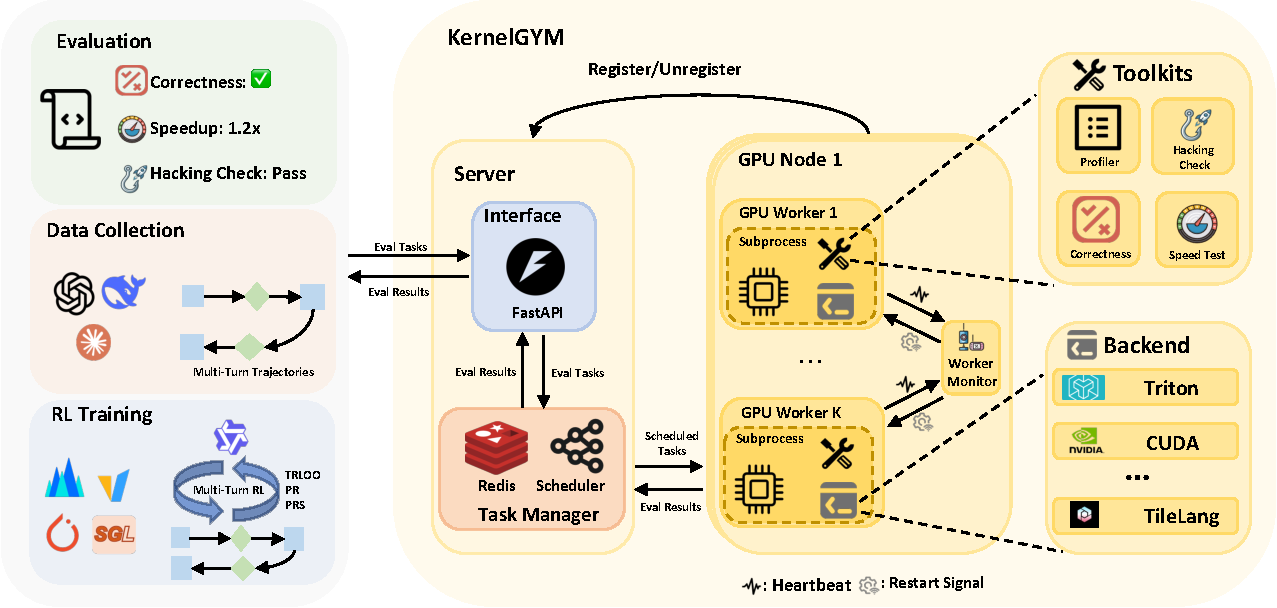
\includegraphics[width=0.9\textwidth]{figures/figure1.pdf}
    \vspace{-6pt}
    \caption{
    Overview of \env{} and our training framework. \textbf{Left:} We study RL training methods for kernel generation, including multi-turn RL with TRLOO, profiling-based rewards (PR), and profiling-based rejection sampling (PRS).
    \textbf{Right:} The architecture of \env{}: a server-worker split distributed design. The server side (interface + task manager) receives evaluation jobs and schedules to registered distributed GPU workers; each job runs in an isolated subprocess; toolkits produce structured signals for training, parallel evaluation and data collections.
    }
    \label{fig:overview}
\end{figure}
\emph{Correctness} and \emph{ speedup} are the two objectives of kernel generation. However, triton kernel generation is particularly vulnerable to \emph{reward hacking}~\citep{baronio2025kevinmultiturnrlgenerating,woo2025tritonrltrainingllmsthink}: the model can produce outputs that appear correct and fast under the evaluation while being actually meaningless. A simple example is copying the Torch reference implementation, it passes correctness checks but yields only $\sim$1.0$\times$ speedup, providing an easy way to harvest reward without learning kernel generation. Another common failure mode occurs when Triton kernels are emitted but never executed in the kernel entry function, resulting in misleading timing measurements. As shown in Figure~\ref{fig:pitfalls} (right), although the model generates the kernel implementation for LayerNorm, the kernel is never actually executed. 

Beyond hacking, we observe a second bottleneck that is specific to \emph{performance}-oriented kernel generation. In Figure~\ref{fig:pitfalls} (Left), we validate Fast@1 and Fast@1.2 on KernelBench Level 2 during training. Fast@1 / Fast@1.2 represent the fraction of kernels passing correctness checks with at least $1\times / 1.2\times$ speedup over the Torch reference. Fast@1 improves steadily, while the stricter Fast@1.2 saturates quickly (around $\sim$100 steps). Unlike standard code generation, where functional correctness is often the end goal, kernel generation ultimately targets \emph{meaningful speedup}. Many KernelBench~\citep{ouyang2025kernelbench} tasks admit trivial-but-correct implementations (e.g., local rewrites such as swapping a simple activation) that do not address the true runtime bottlenecks. As shown in Figure~\ref{fig:pitfalls} (right), the model leverages the kernel for the simple summation operation, while leaving other operations to the Torch implementation, thereby overlooking the potential benefits of more advanced fusion optimizations. Since these solutions still yield only $\sim1\times$ speedup, the policy tends to exploit such low-hanging fruits to improve Fast@1, without producing kernels that clear the higher bar required by Fast@1.2. We refer to this behavior as \emph{lazy optimization}. Cases are provided in Figure~\ref{fig:pitfalls} (Right) and Appendix~\ref{ap:cases:profiling-lazy-optim}.

\wl{Modified} These two issues are also evident and remain unresolved in previous works. For instance, in AutoTriton~\citep{li2025autotriton}, despite implementing a rule-based reward that assigns 0 reward to code without the ``@triton.jit'' decorator, the model still encounters hacking cases, such as neglecting to call the function, as shown in Figure~\ref{fig:pitfalls}. In our evaluation, code generated by their released model still exhibits approximately $10\%$ hacking cases in the KernelBench level-1 subset. In addition to reward hacking, the issue of lazy optimization persists. As shown in Table~\ref{tab:main_table}, while AutoTriton achieves a notable $30.6\%$ performance on the Fast@1 metric in the Kernelbench level-2 subset, its performance on the stricter Fast@1.2 metric quickly saturates to just only $9.2\%$.

Next, to make RL for kernel generation practically feasible, we start with a robust execution environment with hacking checks and torch profiler (\S~\ref{sec:kernelgym}), then introduce an unbiased multi-turn RL estimator (\S~\ref{sec:rl}), and finally improve training stability and align optimization objectives toward real speedup to alleviate lazy optimization (\S~\ref{sec:trade-off-rl}).